\documentclass{warpdoc}
\newlength\lengthfigure                  % declare a figure width unit
\setlength\lengthfigure{0.158\textwidth} % make the figure width unit scale with the textwidth
\usepackage{psfrag}         % use it to substitute a string in a eps figure
\usepackage{subfigure}
\usepackage{rotating}
\usepackage{pstricks}
\usepackage[innercaption]{sidecap} % the cute space-saving side captions
\usepackage{scalefnt}
\usepackage{bm}
\usepackage{amsmath}     
\usepackage{multirow}
\usepackage{graphicx}
\usepackage{rotating}
\usepackage{bm}
\usepackage{pdfpages}
%\usepackage{caption}
\usepackage{float}
\pdfminorversion=7

%%%%%%%%%%%%%=--NEW COMMANDS BEGINS--=%%%%%%%%%%%%%%%%%%%%%%%%%%%%%%%%%%
\newcommand{\alb}{\vspace{0.2cm}\\} % array line break
\newcommand{\ordi}{{\rm d}}
%\let\vec\bf
\renewcommand{\vec}[1]{\bm{#1}}
\newcommand{\mfa}{\scriptscriptstyle}
\newcommand{\mfb}{\scriptstyle}
\newcommand{\mfc}{\textstyle}
\newcommand{\mfd}{\displaystyle}
\newcommand{\hlinex}{\vspace{-0.34cm}~~\\ \hline \vspace{-0.31cm}~~\\}
\newcommand{\hlinextop}{\vspace{-0.46cm}~~\\ \hline \hline \vspace{-0.32cm}~~\\}
\newcommand{\hlinexbot}{\vspace{-0.37cm}~~\\ \hline \hline \vspace{-0.50cm}~~\\}
\newcommand{\tablespacing}{\vspace{-0.4cm}}
\renewcommand{\fontsizetable}{\footnotesize\scalefont{0.9}}
\setcounter{tocdepth}{3}
\let\citen\cite

%%%%%%%%%%%%%=--NEW COMMANDS ENDS--=%%%%%%%%%%%%%%%%%%%%%%%%%%%%%%%%%%%%
%%%%%%%%%%%%%=--NEW COMMANDS BEGINS--=%%%%%%%%%%%%%%%%%%%%%%%%%%%%%%%%%%


\author{
 Felipe Martín Rodríguez Fuentes
}

\email{
  fmrodriguez@arizona.edu
}

\department{
  Aerospace and Mechanical Engineering
}

\institution{
  University of Arizona
}

\title{Eight Species Argon Plasma Kinetics 
}

\date{
Octorber 2025
}

%\setlength\nomenclaturelabelwidth{0.13\hsize}  % optional, default is 0.03\hsize
%\setlength\nomenclaturecolumnsep{0.09\hsize}  % optional, default is 0.06\hsize

\nomenclature{

  \begin{nomenclaturelist}{Roman symbols}
   \item[$a$] speed of sound
  \end{nomenclaturelist}
}


\abstract{
abstract
}

\begin{document}
  \pagestyle{headings}
  \pagenumbering{arabic}
  \setcounter{page}{1}
%  \maketitle
  \makewarpdoctitle
%  \makeabstract
 \tableofcontents
%  \makenomenclature
 % \listoftables
 % \listoffigures
%

\section{Overview}

\begin{table*}[!ht]
  \center\fontsizetable
  \begin{threeparttable}
    \tablecaption{Species included in the reaction mechanism.}
    \label{tab:species}
    \fontsizetable
 
    \begin{tabular*}{0.3\textwidth}{@{}l@{\extracolsep{\fill}}l@{}}
    
    \toprule

charged${}^-$ & $\rm e^-$\\

charged${}^+$ & $\rm Ar^+$, $\rm Ar_2^+$\\
      
neutral, atomic & $\rm Ar$, $\rm Ar(4s)$, $\rm Ar(4p)$\\
      
neutral, molecular & $\rm Ar_2^\star$, $\rm Ar_2$\\

    \bottomrule
    \end{tabular*}
   \end{threeparttable}
\end{table*}

\begin{figure}[ht]
     \centering
     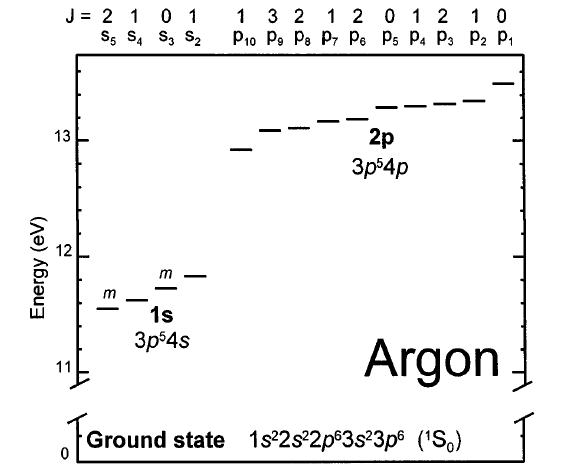
\includegraphics[width=0.5\textwidth]{figs/argon_atomics.png}
     \caption{Energy level diagram for Ar showing the first two
excited configurations. The two metastable levels are indicated
by the letter. The Paschen designation for each level is
indicated at the top of the table. Diagram taken from \cite{pr:1998:piech}.}
     \label{fig:atomdata}
\end{figure}

For the Ar(4s) states, these are lumped together. The statistical weight $g$ is required for the BOLSIG+ superelastic rate calculations. This would be:

$$g = \sum (2J+1) = 5 + 3 + 1 + 3 = 12$$

\begin{figure}[ht]
     \centering
     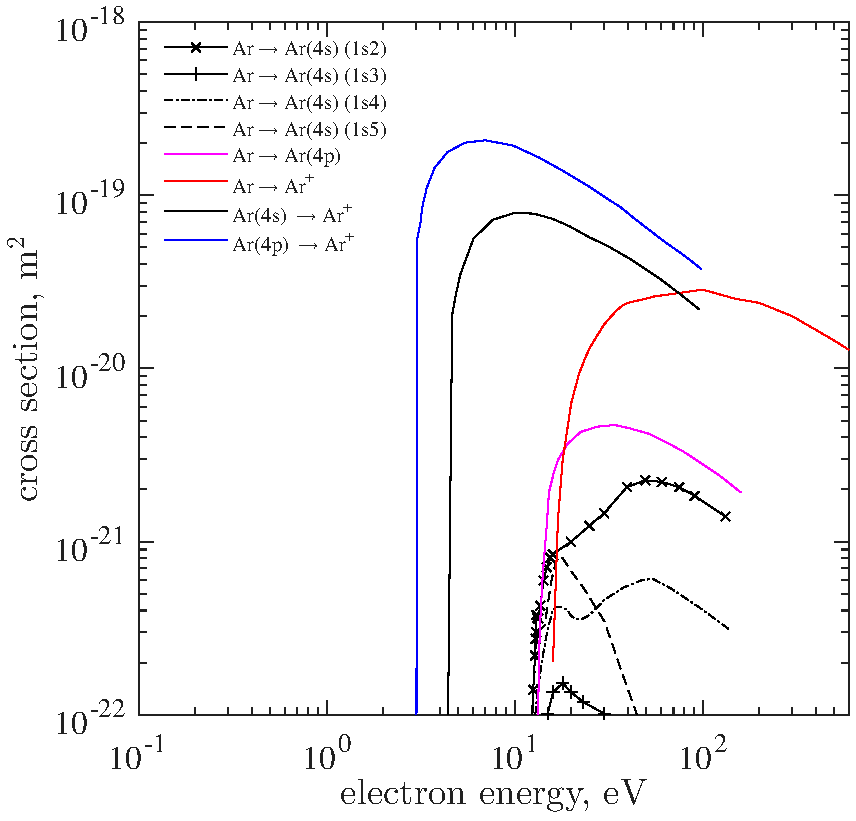
\includegraphics[width=0.5\textwidth]{figs/cs.pdf}
     \caption{Relevant cross sections used for the BOLSIG+ calculations.}
     \label{fig:cs_Ar}
\end{figure}


\section{Argon chemical reactions}

 The list of reactions is given in Table~\ref{tab:Ar_tab}. When reaction rate data is given as a function of the reduced electric field $E/N$, this is converted to reaction rates function of electron energy (or temperature) through the characteristic Ar energy curve $E/N = f(T_{\rm e})$ at 300 K. \cite{ijae:2011:katsonis}, \cite{jap:1993:lymberopoulos}

\begin{figure}[ht]
     \centering
     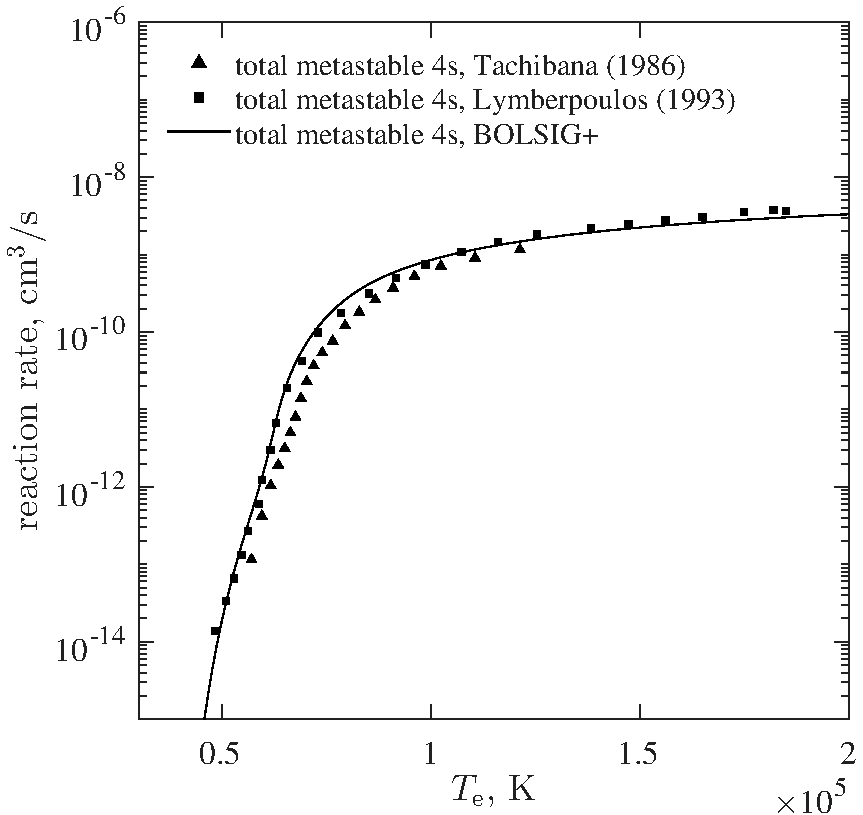
\includegraphics[width=0.5\textwidth]{figs/reaction1.pdf}
     \caption{Reaction 1: $\rm e^- + Ar \leftrightarrow Ar(4s) + e^-$; comparison of total excitation and superelastic rates to 4s levels of Argon obtained with BOLSIG+ using cross section data from \cite{pr:tachibana:1986} at 300 K. Spline fitted to BOLSIG+ data.}
     \label{fig:rate_R1}
\end{figure}

\begin{figure}[ht]
     \centering
     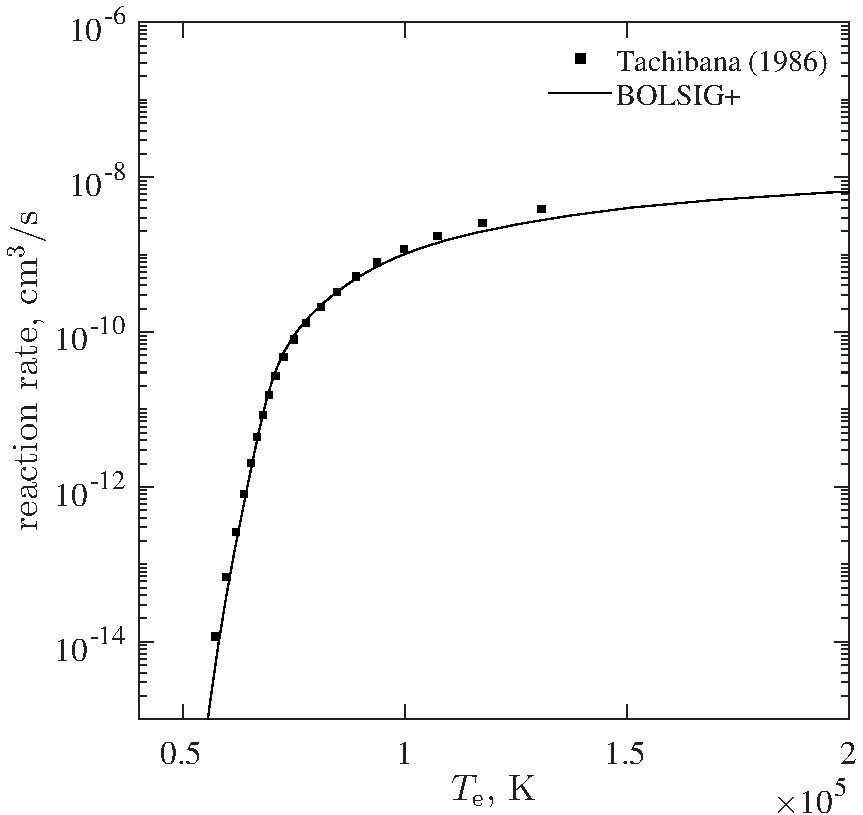
\includegraphics[width=0.5\textwidth]{figs/reaction2.pdf}
     \caption{Reaction 2: $\rm e^- + Ar \rightarrow Ar(4p) + e^-$; comparison of total excitation and superelastic rates to 4p levels of Argon obtained with BOLSIG+ using cross section data from \cite{pr:tachibana:1986} at 300 K. Spline fitted to BOLSIG+ data.}
     \label{fig:rate_R2}
\end{figure}

\begin{figure}[ht]
     \centering
     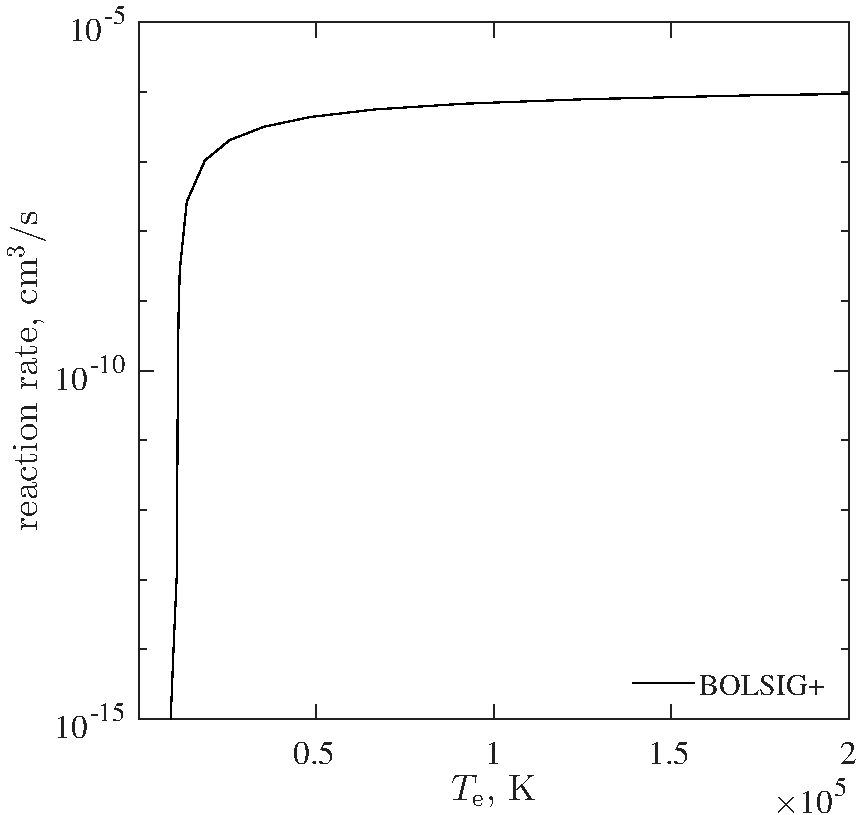
\includegraphics[width=0.5\textwidth]{figs/reaction3.pdf}
     \caption{Reaction 2: $\rm e^- + Ar(4s) \rightarrow Ar(4p) + e^-$; comparison of total excitation rate from 4s to 4p levels of Argon obtained with BOLSIG+ using cross section data from \cite{pr:2014:zatsarinny} at 300 K. Spline fitted to BOLSIG+ data.}
     \label{fig:rate_R3}
\end{figure}

\begin{figure}[ht]
     \centering
     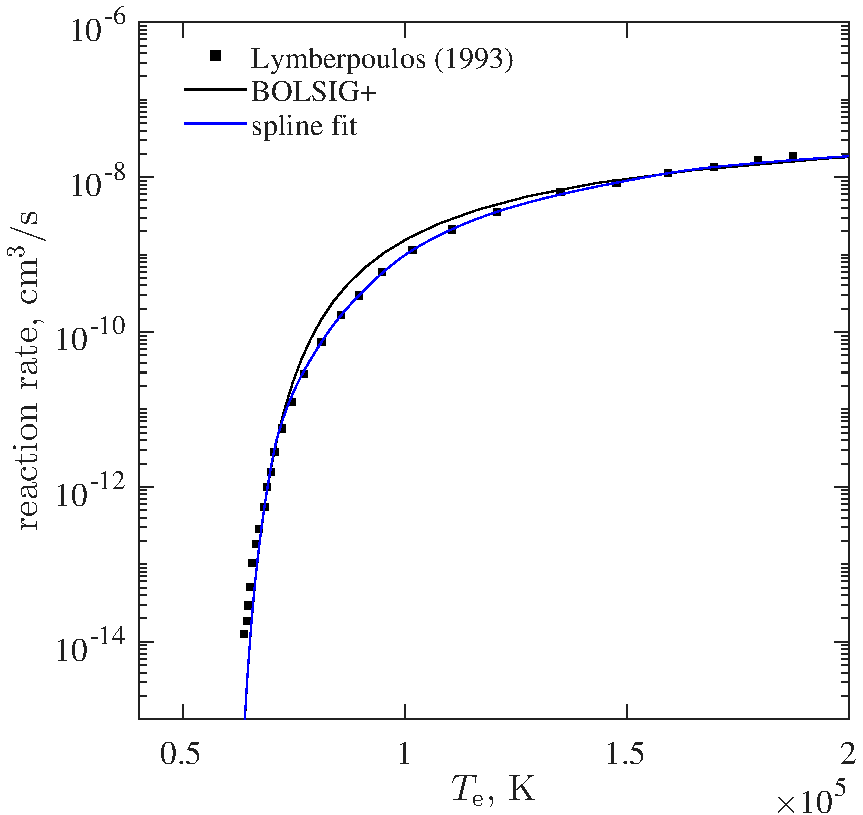
\includegraphics[width=0.5\textwidth]{figs/reaction4.pdf}
     \caption{Reaction 4: $\rm e^- + Ar \rightarrow Ar^+ + 2e^-$; comparison of ionization rate of Ar obtained with BOLSIG+ using cross section data from \cite{jcp:1965:rapp} at 300 K. Reference data from \cite{jap:1993:lymberopoulos, pop:2012:adams}.}
     \label{fig:rate_R4}
\end{figure}

\begin{figure}[ht]
     \centering
     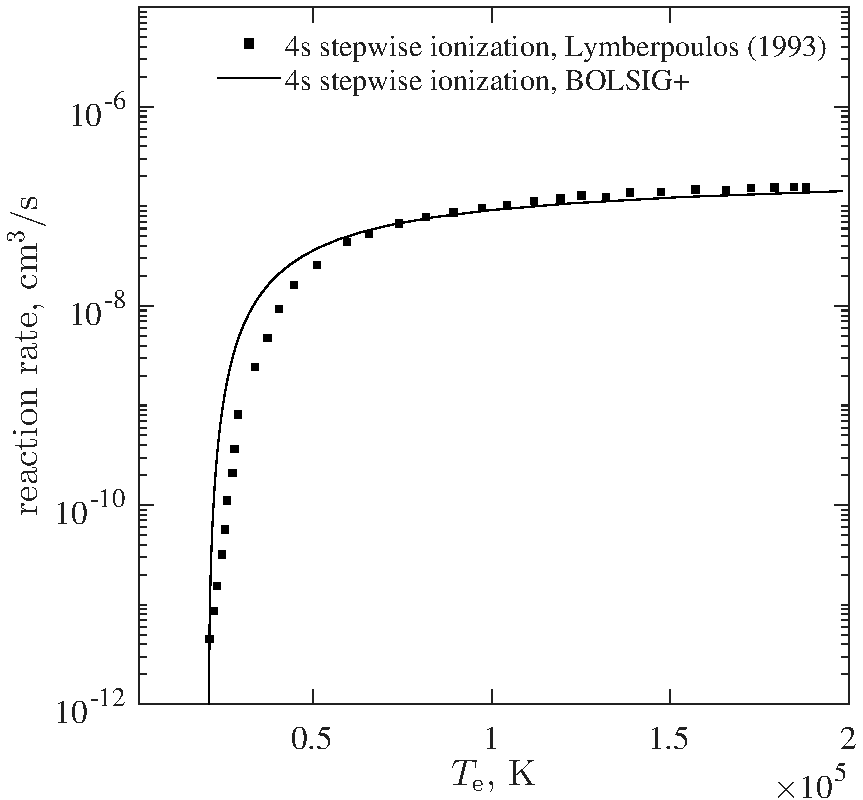
\includegraphics[width=0.5\textwidth]{figs/reaction5.pdf}
     \caption{Reaction 5: $\rm e^- + Ar(4s) \rightarrow Ar^+ + 2e^-$; comparison of ionization rate of Ar(4s) obtained with BOLSIG+ using cross section data from \cite{pr:hyman:1979} at 300 K. Spline fitted to BOLSIG+ data.}
     \label{fig:rate_R5}
\end{figure}

\begin{figure}[ht]
     \centering
     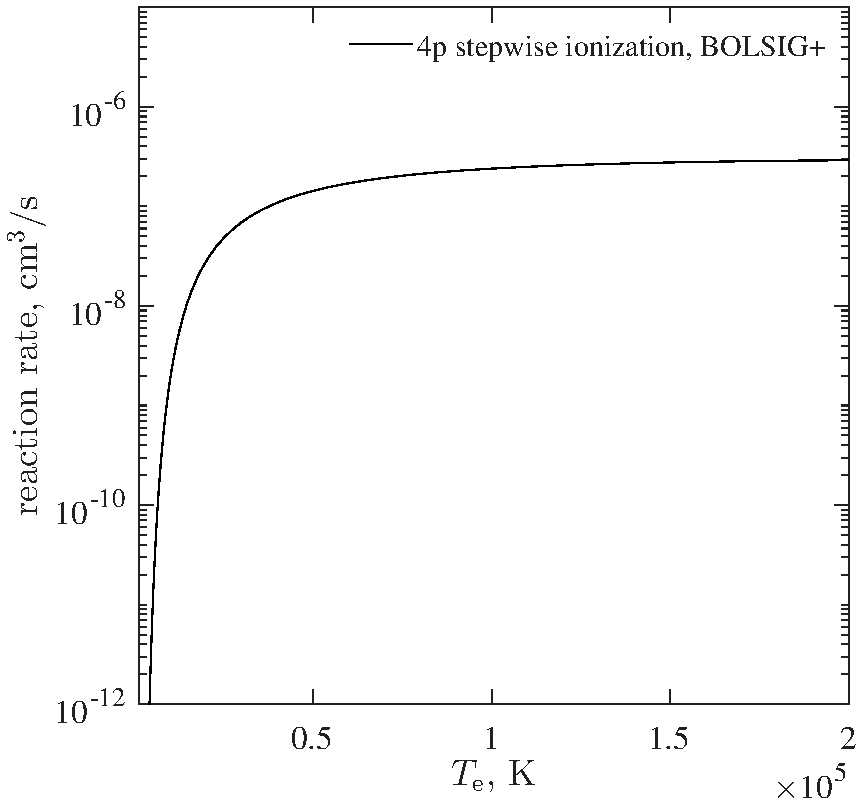
\includegraphics[width=0.5\textwidth]{figs/reaction6.pdf}
     \caption{Reaction 5: $\rm e^- + Ar(4p) \rightarrow Ar^+ + 2e^-$; comparison of ionization rate of Ar(4p) obtained with BOLSIG+ using cross section data from \cite{pr:hyman:1979} at 300 K. Spline fitted to BOLSIG+ data.}
     \label{fig:rate_R6}
\end{figure}

% \section{Electron swarm parameters in Argon gas at 300 K}

% \subsection{Reduced electric field function of electron temperature (local approximation)}

% \begin{figure}[ht]
%      \centering
%      \includegraphics[width=0.5\textwidth]{figs/Estar_Te.pdf}
%      \caption{Reduced electric field function of electron temperature for Argon gas at 300 K. Comparisons with data from refs. \cite{ajp:1977:milloy} and \cite{pr:1995:boeuf}.}
%      \label{fig:estar_te}
% \end{figure}

% \subsection{Reduced electron mobility function of electron temperature}


% \begin{figure}[ht]
%      \centering
%      \includegraphics[width=0.5\textwidth]{figs/mueN_Te.pdf}
%      \caption{Reduced electron mobility function of electron temperature for Argon gas at 300 K. Comparisons with data from refs. \cite{pr:1961:pack}, \cite{purdue:1951:errett} and \cite{jop:1981:kucukarpaci}.}
%      \label{fig:muen_te}
% \end{figure}













\begin{table*}[!ht]
  \center\fontsizetable
  \begin{threeparttable}
  \renewcommand{\arraystretch}{1.1}
    \tablecaption{Argon chemical kinetics\tnote{a}.}
    \label{tab:Ar_tab}
    \fontsizetable
    \begin{tabular*}{1.05\textwidth}{l@{\extracolsep{\fill}}lllccr}
    \toprule
    No.~~~~& Reaction & $T,~\textrm{K}$ & $A$  & $n$ & $E$ & Cross-section ref. \\
    \midrule

  
% \multicolumn{3}{p{3cm}}{Electron impact reactions} 
%        & 
%        & 
%        & \\     
%    \midrule
    
     1  & $\rm e^- +Ar \leftrightarrow Ar(4s) + e^-$
       & $T_{\rm e}$
       & \multicolumn{3}{p{6cm}}{Rates obtained with BOLSIG+ and detailed balance}
       & \cite{pr:tachibana:1986}\\   


2  & {$\rm e^- +Ar \leftrightarrow Ar(4p) + e^-$}
       & $T_{\rm e}$
      & \multicolumn{3}{p{6cm}}{Rates obtained with BOLSIG+ and detailed balance}  
       & \cite{pr:tachibana:1986}\\


    3 & $\rm e^- +Ar(4s) \leftrightarrow Ar(4p) + e^-$
       & $T_{\rm e}$
      & \multicolumn{3}{p{6cm}}{Rates obtained with BOLSIG+ and detailed balance}  
       & \cite{pr:2014:zatsarinny}\\


  4  & $\rm e^- +Ar \rightarrow Ar^+ + e^- + e^-$
       & $T_{\rm e}$
       & \multicolumn{3}{p{6cm}}{Rate obtained with BOLSIG+}       
       & \cite{jcp:1965:rapp} \\

    5  & $\rm e^- +Ar(4s) \rightarrow Ar^+ + e^- + e^-$
       & $T_{\rm e}$
       & \multicolumn{3}{p{6cm}}{Rate obtained with BOLSIG+}       
       & \cite{pr:hyman:1979} \\

    6  & $\rm e^- +Ar(4p) \rightarrow Ar^+ + e^- + e^-$
       & $T_{\rm e}$
       & \multicolumn{3}{p{6cm}}{Rate obtained with BOLSIG+}       
       & \cite{pr:hyman:1979} \\

   % 7  & $\rm e^- +Ar_2^\star \rightarrow Ar_2^+ + e^- + e^-$
   %     & $T_{\rm e}$ 
   %     & \multicolumn{3}{p{8cm}}{$9.0\cdot10^{-8}\cdot T_{\rm e}^{0.7}\cdot \exp (-3.66/T_{\rm e})~~\rm cm^3/s$}       
   %     & \cite{jof:2007:arakoni} \\

   7  & $\rm e^- +Ar_2^\star \rightarrow Ar_2^+ + e^- + e^-$
       & $T_{\rm e}$ in eV
       & $9.0\cdot10^{-8}\cdot N_A$  
       &0.7
       &$3.66R$   
       & \cite{jof:2007:arakoni} \\

   8  & $\rm e^- +Ar_2^\star \rightarrow Ar + Ar + e^-$
       & $T_{\rm e}$ in eV
       & $1.0\cdot10^{-7}\cdot N_A$
                       &0.0
       &0.0   
       & \cite{jof:2007:arakoni} \\

   9  & $\rm e^- +Ar_2^+ \rightarrow Ar(4p) + Ar$
       & $T_{\rm e}$  in eV
       & $5.4\cdot10^{-8}\cdot N_A$
                   &-0.66
       &0.0   
       & \cite{jof:2007:arakoni} \\

          10  & $\rm e^- +Ar^+ \rightarrow Ar(4p) $
       & $T_{\rm e}$ in eV
       & $4.0\cdot10^{-13}\cdot N_A$
               &-0.50
       &0.0   
       & \cite{jof:2007:arakoni} \\

       
          11 & $\rm e^- + e^- +Ar^+ \rightarrow Ar(4p) + e^- $
       & $T_{\rm e}$ in eV
       & $5.0\cdot10^{-27}\cdot N_A^2$ 
        &-4.50
       &0.0   
       & \cite{jof:2007:arakoni} \\

   \midrule
\multicolumn{3}{p{3cm}}{Penning ionization} 
       & 
       & 
       & \\     
   \midrule

          12 & $\rm Ar(4s) + Ar(4s) \rightarrow Ar^+ +Ar + e^- $
       & $T$ 
       & $1.0\cdot10^{-9}\cdot N_A $    
       &0.0
       &0.0       
       & \cite{jof:2007:arakoni} \\

          13 & $\rm Ar(4s) + Ar(4p) \rightarrow Ar^+ +Ar + e^- $
       & $T$ 
       & $1.0\cdot10^{-9}\cdot N_A $    
       &0.0
       &0.0
       & \cite{jof:2007:arakoni} \\

          14 & $\rm Ar(4p) + Ar(4p) \rightarrow Ar^+ +Ar + e^- $
       & $T$ 
       & $1.0\cdot10^{-9}\cdot N_A $    
       &0.0
       &0.0   
       & \cite{jof:2007:arakoni} \\


          15 & $\rm Ar_2^\star + Ar_2^\star \rightarrow Ar_2^+ +Ar + Ar + e^- $
       & $T$ 
       & $5.0\cdot10^{-10}\cdot N_A $    
       &0.0
       &0.0 
       & \cite{ieee:2003:kannari} \\
          \midrule
\multicolumn{3}{p{3cm}}{Three-body neutral reactions} 
       & 
       & 
       & \\     
   \midrule
         16 & $\rm Ar(4s) + Ar + Ar \rightarrow Ar_2^\star +Ar $
       & $T$ 
       & $1.0\cdot10^{-32}\cdot N_A^2 $    
       &0.0
       &0.0     
       & \cite{jof:2007:arakoni} \\

          17 & $\rm Ar(4p) + Ar + Ar \rightarrow Ar_2^\star +Ar $
       & $T$ 
       & $1.0\cdot10^{-32}\cdot N_A^2 $    
       &0.0
       &0.0         
       & \cite{jof:2007:arakoni} \\
          \midrule
\multicolumn{3}{p{3cm}}{Charge transfer} 
       & 
       & 
       & \\     
   \midrule
          18 & $\rm Ar^+ + Ar + Ar \rightarrow Ar_2^+ +Ar $
       & $T$ 
       & $2.5\cdot10^{-31}\cdot N_A^2$
     &0.0
       &0.0    
       & \cite{ieee:2003:kannari} \\

 
    \bottomrule
    \end{tabular*}
\begin{tablenotes}
\item[{a}] The reaction rate is given by $A T^n \exp(-E/RT)$ when not presented in spline-fit form. The universal gas constant is $R = 1.987~{\rm cal~K^{-1}~mol^{-1}}.$ $N_A$ is Avogadro's number and it is approximately $6.022 \cdot 10^{23}~{\rm mol^{-1}}$. The units of $A$ are $\rm cm^3~ mol^{-1} ~s^{-1}$ for 2-body reactions and $\rm cm^6 ~mol^{-2} ~ s^{-1}$ for 3-body reactions. The units of $E$ are ${\rm cal~mol^{-1}}$.
% \item[{b}] The third body species $\rm M^+$ are all positive ions. Efficiencies are set to 1.0 for all species involved.
% \item[{c}] The third body species M are $\rm NH_3$, $\rm NH_3$$(v)$, $\rm NH_2$ and $\rm NH$ with the  corresponding positive ions. Efficiencies are set to 1.0 for all species involved.

\end{tablenotes}
   \end{threeparttable}
\end{table*}


\begin{table*}[!ht]
  \center\fontsizetable
  
  \begin{threeparttable}
    \tablecaption{Coordinates of spline control points for Argon electron impact reactions.\tnote{a}}
    \label{tab:ei_splines_Ar}
    \fontsizetable
 
    \begin{tabular*}{\textwidth}{@{}l@{\extracolsep{\fill}}lll@{}}
    
    \toprule
Process & Reaction ~ & ${\rm ln}~T_{\rm e}$ & ${\rm ln}~k$ \\
        \midrule
        

Ground Excitation & ~{$\rm e^- + Ar \rightarrow Ar(4s) + e^- + e^-$  } &   \begin{minipage}[t]{0.28\textwidth}\raggedright  
      10.4268
      10.4485
      10.4702
      10.4919
      10.5135
      10.5352
      10.5569
      10.6648
      10.7727
      10.8755
      10.9536
      11.0001
      11.0270
      11.0510
      11.0942
      11.1474
      11.2135
      11.2963
      11.4088
      11.5797
      11.8688
      12.4147
      13.2881
 \end{minipage}  & \begin{minipage}[t]{0.28\textwidth}\raggedright 
      -56.8696
      -54.4046
      -52.1035
      -49.9593
      -47.9647
      -46.1123
      -44.3839
      -37.5377
      -33.0186
      -30.1382
      -28.3493
      -27.2040
      -26.3998
      -25.6123
      -24.4623
      -23.5214
      -22.6969
      -21.9640
      -21.3009
      -20.6658
      -20.0016
      -19.3066
      -18.7517
\end{minipage} \\         
~\\

Ground Excitation & ~{$\rm e^- + Ar \rightarrow Ar(4p) + e^- + e^-$  } &   \begin{minipage}[t]{0.28\textwidth}\raggedright  
      10.5458
      10.5516
      10.5634
      10.5810
      10.6173
      10.6391
      10.6609
      10.6827
      10.7045
      10.7263
      10.7568
      10.8482
      10.9395
      11.0309
      11.1223
      11.2136
      11.3050
      11.6849
      12.1191
      12.5532
      12.9874
      13.4216
      13.8557
 \end{minipage}  & \begin{minipage}[t]{0.28\textwidth}\raggedright 
      -59.8263
      -57.1625
      -55.4644
      -53.6640
      -50.3979
      -48.6135
      -46.9705
      -45.4405
      -44.0279
      -42.7250
      -41.0624
      -36.9853
      -33.5895
      -29.3102
      -25.0301
      -23.1149
      -21.9900
      -20.0091
      -19.1682
      -18.7410
      -18.4801
      -18.3097
      -18.2066
\end{minipage} \\         
~\\
4s-4p Excitation & ~{$\rm e^- + Ar(4s) \rightarrow Ar(4p) + e^- + e^-$  } &   \begin{minipage}[t]{0.28\textwidth}\raggedright  
8.6415
8.6660
8.7284
8.8483
8.8827
8.9692
9.2003
9.3069
9.3600
9.8355
10.4707
11.1059
11.7411
12.3763
13.0115
13.6467
 \end{minipage}  & \begin{minipage}[t]{0.28\textwidth}\raggedright 
-55.1215
-53.6653
-50.0461
-43.7516
-42.1551
-38.6210
-32.1118
-24.5656
-19.7036
-16.0787
-14.9664
-14.3921
-14.0539
-13.8157
-13.6388
-13.5296
\end{minipage} \\         
~\\


Ground ionization & ~{$\rm e^- + Ar \rightarrow Ar^+ + e^- + e^-$  } &   \begin{minipage}[t]{0.28\textwidth}\raggedright  

10.8750
10.9124
10.9498
11.0114
11.0455
11.0726
11.1022
11.1367
11.1764
11.3050
11.4034
11.5300
11.7013
11.9025
12.0413
12.6518
12.9347
13.2406
13.5674
13.9179
 \end{minipage}  & \begin{minipage}[t]{0.28\textwidth}\raggedright 
-58.8256
-55.3326
-51.6404
-43.8976
-37.8100
-33.5388
-30.3825
-27.9742
-26.0716
-23.3203
-21.9406
-20.5902
-19.4518
-18.5862
-18.1199
-17.2191
-16.9601
-16.7451
-16.5707
-16.4356


\end{minipage} \\         
~\\


Step. ionization & ~{$\rm e^- + Ar(4s) \rightarrow Ar^+ + e^- + e^-$  } &   \begin{minipage}[t]{0.28\textwidth}\raggedright  
      8.9802
      9.0676
      9.1551
      9.2425
      9.3299
      9.4174
      9.8546
      10.2918
      10.7290
      11.1662
      11.6034
      12.0406
      12.4778
      12.9150
      13.3522
      13.7894
 \end{minipage}  & \begin{minipage}[t]{0.28\textwidth}\raggedright 
      -47.4567
      -42.7722
      -38.2715
      -34.2096
      -30.8706
      -28.2804
      -21.6398
      -18.7954
      -17.3209
      -16.5828
      -16.1777
      -15.9052
      -15.6982
      -15.5401
      -15.4256
      -15.3526
\end{minipage} \\ 
~\\

Step. ionization & ~{$\rm e^- + Ar(4p) \rightarrow Ar^+ + e^- + e^-$  } &   \begin{minipage}[t]{0.28\textwidth}\raggedright  
      7.0565
      7.1440
      7.2314
      7.3188
      7.4063
      7.4937
      7.9309
      8.3681
      8.8053
      9.2425
      9.6797
      10.1169
      10.5541
      10.9913
      11.4285
      11.8657
      12.3029
      12.7401
      13.1773
      13.6145
 \end{minipage}  & \begin{minipage}[t]{0.28\textwidth}\raggedright 
      -59.6786
      -55.9265
      -52.4893
      -49.3405
      -46.4559
      -43.8130
      -33.5699
      -26.9462
      -22.6538
      -19.8643
      -18.0459
      -16.8581
      -16.0849
      -15.5899
      -15.2858
      -15.1149
      -15.0390
      -15.0317
      -15.0730
      -15.1476
\end{minipage} \\ 
 \alb 
    \bottomrule
    \end{tabular*}
\begin{tablenotes}
\item[{a}] The reaction rate $k$ has units of $\textrm{cm}^3\cdot \textrm{s}^{-1}$. The electron temperature $T_{\rm e}$ is in Kelvin.

\end{tablenotes}
\label{tab:reactionratessplinecontrolpoints}
   \end{threeparttable}
\end{table*}


% \section{GEC Reference Reactor Validation Results}


 \clearpage
\bibliographystyle{warpdoc}
\bibliography{all}


\end{document}


